% inspired from http://www.texample.net/tikz/examples/merge-sort-recursion-tree/
\documentclass{article}

\usepackage[utf8]{inputenc}
\usepackage[T1]{fontenc}
\usepackage{tikz}
\usetikzlibrary{shapes, positioning, arrows, calc}
\usetikzlibrary{decorations.pathreplacing}

\begin{document}

% Exemple dichotomie

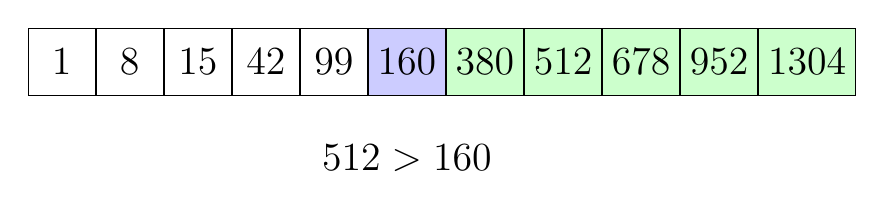
\begin{tikzpicture}
   \node [font=\sffamily\Large\bfseries, draw, anchor=center, minimum size=0.85cm] (first) {$1$};
   \node [font=\sffamily\Large\bfseries, draw, anchor=center, right=0cm of first, minimum size=0.85cm] (second) {$8$};
   \node [font=\sffamily\Large\bfseries, draw, anchor=center, right=0cm of second, minimum size=0.85cm] (third) {$15$};
   \node [font=\sffamily\Large\bfseries, draw, anchor=center, right=0cm of third, minimum size=0.85cm] (fourth) {$42$};
   \node [font=\sffamily\Large\bfseries, draw, anchor=center, right=0cm of fourth, minimum size=0.85cm] (fifth) {$99$};
   \node [font=\sffamily\Large\bfseries, draw, anchor=center, right=0cm of fifth, minimum size=0.85cm, fill=blue!20] (sixth) {$160$};
   \node [font=\sffamily\Large\bfseries, draw, anchor=center, right=0cm of sixth, minimum size=0.85cm, fill=green!20] (seventh) {$380$};
   \node [font=\sffamily\Large\bfseries, draw, anchor=center, right=0cm of seventh, minimum size=0.85cm, fill=green!20] (eighth) {$512$};
   \node [font=\sffamily\Large\bfseries, draw, anchor=center, right=0cm of eighth, minimum size=0.85cm, fill=green!20] (ninth) {$678$};
   \node [font=\sffamily\Large\bfseries, draw, anchor=center, right=0cm of ninth, minimum size=0.85cm, fill=green!20] (tenth) {$952$};
   \node [font=\sffamily\Large\bfseries, draw, anchor=center, right=0cm of tenth, minimum size=0.85cm, fill=green!20] (eleventh) {$1304$};

   \node [font=\sffamily\Large\bfseries, anchor=center, below=0.5cm of sixth] (text) {$512 > 160$};
\end{tikzpicture}

\vspace{0.5cm}

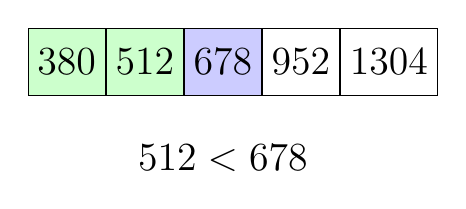
\begin{tikzpicture}
   \node [font=\sffamily\Large\bfseries, draw, anchor=center, minimum size=0.85cm, fill=green!20] (first) {$380$};
   \node [font=\sffamily\Large\bfseries, draw, anchor=center, right=0cm of first, minimum size=0.85cm, fill=green!20] (second) {$512$};
   \node [font=\sffamily\Large\bfseries, draw, anchor=center, right=0cm of second, minimum size=0.85cm, fill=blue!20] (third) {$678$};
   \node [font=\sffamily\Large\bfseries, draw, anchor=center, right=0cm of third, minimum size=0.85cm] (fourth) {$952$};
   \node [font=\sffamily\Large\bfseries, draw, anchor=center, right=0cm of fourth, minimum size=0.85cm] (fifth) {$1304$};

   \node [font=\sffamily\Large\bfseries, anchor=center, below=0.5cm of third] (text) {$512 < 678$};
\end{tikzpicture}

\vspace{0.5cm}

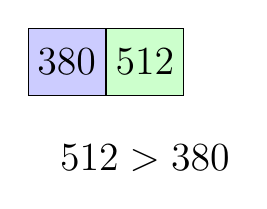
\begin{tikzpicture}
   \node [font=\sffamily\Large\bfseries, draw, anchor=center, minimum size=0.85cm, fill=blue!20] (first) {$380$};
   \node [font=\sffamily\Large\bfseries, draw, anchor=center, right=0cm of first, minimum size=0.85cm, fill=green!20] (second) {$512$};

   \node [font=\sffamily\Large\bfseries, anchor=center, below=0.5cm of second] (text) {$512 > 380$};
\end{tikzpicture}

\vspace{0.5cm}

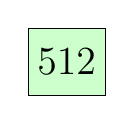
\begin{tikzpicture}
   \node [font=\sffamily\Large\bfseries, draw, anchor=center, minimum size=0.85cm, fill=green!20] (first) {$512$};
\end{tikzpicture}

\newpage

% Calcul complexité recherche dichotomique

% http://www.texample.net/tikz/examples/merge-sort-recursion-tree/
% MergeSort-RecursionTree by Manuel Kirsch

\begin{tikzpicture}[level/.style={sibling distance=50mm/#1}]
   \node [circle,draw] (z){$n$}
   child {node [circle,draw] (a) {$\frac{n}{2}$}
      child {node [circle,draw] (b) {$\frac{n}{2^2}$}
         child {node {$\vdots$}
            child {node [circle,draw] (d) {$\frac{n}{2^k}$}}
            child {node [circle,draw] (e) {$\frac{n}{2^k}$}}
         } 
         child {node {$\vdots$}}
      }
      child {node [circle,draw] (g) {$\frac{n}{2^2}$}
         child {node {$\vdots$}}
         child {node {$\vdots$}}
      }
   }
   child {node [circle,draw] (j) {$\frac{n}{2}$}
      child {node [circle,draw] (k) {$\frac{n}{2^2}$}
         child {node {$\vdots$}}
         child {node {$\vdots$}}
      }
      child {node [circle,draw] (l) {$\frac{n}{2^2}$}
         child {node {$\vdots$}}
         child {node (c){$\vdots$}
            child {node [circle,draw] (o) {$\frac{n}{2^k}$}}
            child {node [circle,draw] (p) {$\frac{n}{2^k}$}
               child [grow=right] {node (q) {$\Rightarrow$} edge from parent[draw=none]
                  child [grow=right] {node (q) {$\log n$} edge from parent[draw=none]
                     child [grow=up] {node (r) {$\vdots$} edge from parent[draw=none]
                        child [grow=up] {node (s) {$3$} edge from parent[draw=none]
                           child [grow=up] {node (t) {$2$} edge from parent[draw=none]
                              child [grow=up] {node (u) {$1$} edge from parent[draw=none]}
                           }
                        }
                     }
                  }
               }
            }
         }
      }
   };

   \path (s) -- (l) node [midway] {$\Rightarrow$};
   \path (z) -- (u) node [midway] {$\Rightarrow$};
   \path (j) -- (t) node [midway] {$\Rightarrow$};
   \path (r) -- (c) node [midway] {$\cdots$};
   \path (e) -- (o) node [midway] {$\cdots$};
\end{tikzpicture}

\end{document}
